% Options for packages loaded elsewhere
% Options for packages loaded elsewhere
\PassOptionsToPackage{unicode}{hyperref}
\PassOptionsToPackage{hyphens}{url}
\PassOptionsToPackage{dvipsnames,svgnames,x11names}{xcolor}
%
\documentclass[
  letterpaper,
  DIV=11,
  numbers=noendperiod]{scrartcl}
\usepackage{xcolor}
\usepackage{amsmath,amssymb}
\setcounter{secnumdepth}{-\maxdimen} % remove section numbering
\usepackage{iftex}
\ifPDFTeX
  \usepackage[T1]{fontenc}
  \usepackage[utf8]{inputenc}
  \usepackage{textcomp} % provide euro and other symbols
\else % if luatex or xetex
  \usepackage{unicode-math} % this also loads fontspec
  \defaultfontfeatures{Scale=MatchLowercase}
  \defaultfontfeatures[\rmfamily]{Ligatures=TeX,Scale=1}
\fi
\usepackage{lmodern}
\ifPDFTeX\else
  % xetex/luatex font selection
\fi
% Use upquote if available, for straight quotes in verbatim environments
\IfFileExists{upquote.sty}{\usepackage{upquote}}{}
\IfFileExists{microtype.sty}{% use microtype if available
  \usepackage[]{microtype}
  \UseMicrotypeSet[protrusion]{basicmath} % disable protrusion for tt fonts
}{}
\makeatletter
\@ifundefined{KOMAClassName}{% if non-KOMA class
  \IfFileExists{parskip.sty}{%
    \usepackage{parskip}
  }{% else
    \setlength{\parindent}{0pt}
    \setlength{\parskip}{6pt plus 2pt minus 1pt}}
}{% if KOMA class
  \KOMAoptions{parskip=half}}
\makeatother
% Make \paragraph and \subparagraph free-standing
\makeatletter
\ifx\paragraph\undefined\else
  \let\oldparagraph\paragraph
  \renewcommand{\paragraph}{
    \@ifstar
      \xxxParagraphStar
      \xxxParagraphNoStar
  }
  \newcommand{\xxxParagraphStar}[1]{\oldparagraph*{#1}\mbox{}}
  \newcommand{\xxxParagraphNoStar}[1]{\oldparagraph{#1}\mbox{}}
\fi
\ifx\subparagraph\undefined\else
  \let\oldsubparagraph\subparagraph
  \renewcommand{\subparagraph}{
    \@ifstar
      \xxxSubParagraphStar
      \xxxSubParagraphNoStar
  }
  \newcommand{\xxxSubParagraphStar}[1]{\oldsubparagraph*{#1}\mbox{}}
  \newcommand{\xxxSubParagraphNoStar}[1]{\oldsubparagraph{#1}\mbox{}}
\fi
\makeatother

\usepackage{color}
\usepackage{fancyvrb}
\newcommand{\VerbBar}{|}
\newcommand{\VERB}{\Verb[commandchars=\\\{\}]}
\DefineVerbatimEnvironment{Highlighting}{Verbatim}{commandchars=\\\{\}}
% Add ',fontsize=\small' for more characters per line
\usepackage{framed}
\definecolor{shadecolor}{RGB}{241,243,245}
\newenvironment{Shaded}{\begin{snugshade}}{\end{snugshade}}
\newcommand{\AlertTok}[1]{\textcolor[rgb]{0.68,0.00,0.00}{#1}}
\newcommand{\AnnotationTok}[1]{\textcolor[rgb]{0.37,0.37,0.37}{#1}}
\newcommand{\AttributeTok}[1]{\textcolor[rgb]{0.40,0.45,0.13}{#1}}
\newcommand{\BaseNTok}[1]{\textcolor[rgb]{0.68,0.00,0.00}{#1}}
\newcommand{\BuiltInTok}[1]{\textcolor[rgb]{0.00,0.23,0.31}{#1}}
\newcommand{\CharTok}[1]{\textcolor[rgb]{0.13,0.47,0.30}{#1}}
\newcommand{\CommentTok}[1]{\textcolor[rgb]{0.37,0.37,0.37}{#1}}
\newcommand{\CommentVarTok}[1]{\textcolor[rgb]{0.37,0.37,0.37}{\textit{#1}}}
\newcommand{\ConstantTok}[1]{\textcolor[rgb]{0.56,0.35,0.01}{#1}}
\newcommand{\ControlFlowTok}[1]{\textcolor[rgb]{0.00,0.23,0.31}{\textbf{#1}}}
\newcommand{\DataTypeTok}[1]{\textcolor[rgb]{0.68,0.00,0.00}{#1}}
\newcommand{\DecValTok}[1]{\textcolor[rgb]{0.68,0.00,0.00}{#1}}
\newcommand{\DocumentationTok}[1]{\textcolor[rgb]{0.37,0.37,0.37}{\textit{#1}}}
\newcommand{\ErrorTok}[1]{\textcolor[rgb]{0.68,0.00,0.00}{#1}}
\newcommand{\ExtensionTok}[1]{\textcolor[rgb]{0.00,0.23,0.31}{#1}}
\newcommand{\FloatTok}[1]{\textcolor[rgb]{0.68,0.00,0.00}{#1}}
\newcommand{\FunctionTok}[1]{\textcolor[rgb]{0.28,0.35,0.67}{#1}}
\newcommand{\ImportTok}[1]{\textcolor[rgb]{0.00,0.46,0.62}{#1}}
\newcommand{\InformationTok}[1]{\textcolor[rgb]{0.37,0.37,0.37}{#1}}
\newcommand{\KeywordTok}[1]{\textcolor[rgb]{0.00,0.23,0.31}{\textbf{#1}}}
\newcommand{\NormalTok}[1]{\textcolor[rgb]{0.00,0.23,0.31}{#1}}
\newcommand{\OperatorTok}[1]{\textcolor[rgb]{0.37,0.37,0.37}{#1}}
\newcommand{\OtherTok}[1]{\textcolor[rgb]{0.00,0.23,0.31}{#1}}
\newcommand{\PreprocessorTok}[1]{\textcolor[rgb]{0.68,0.00,0.00}{#1}}
\newcommand{\RegionMarkerTok}[1]{\textcolor[rgb]{0.00,0.23,0.31}{#1}}
\newcommand{\SpecialCharTok}[1]{\textcolor[rgb]{0.37,0.37,0.37}{#1}}
\newcommand{\SpecialStringTok}[1]{\textcolor[rgb]{0.13,0.47,0.30}{#1}}
\newcommand{\StringTok}[1]{\textcolor[rgb]{0.13,0.47,0.30}{#1}}
\newcommand{\VariableTok}[1]{\textcolor[rgb]{0.07,0.07,0.07}{#1}}
\newcommand{\VerbatimStringTok}[1]{\textcolor[rgb]{0.13,0.47,0.30}{#1}}
\newcommand{\WarningTok}[1]{\textcolor[rgb]{0.37,0.37,0.37}{\textit{#1}}}

\usepackage{longtable,booktabs,array}
\newcounter{none} % for unnumbered tables
\usepackage{calc} % for calculating minipage widths
% Correct order of tables after \paragraph or \subparagraph
\usepackage{etoolbox}
\makeatletter
\patchcmd\longtable{\par}{\if@noskipsec\mbox{}\fi\par}{}{}
\makeatother
% Allow footnotes in longtable head/foot
\IfFileExists{footnotehyper.sty}{\usepackage{footnotehyper}}{\usepackage{footnote}}
\makesavenoteenv{longtable}
\usepackage{graphicx}
\makeatletter
\newsavebox\pandoc@box
\newcommand*\pandocbounded[1]{% scales image to fit in text height/width
  \sbox\pandoc@box{#1}%
  \Gscale@div\@tempa{\textheight}{\dimexpr\ht\pandoc@box+\dp\pandoc@box\relax}%
  \Gscale@div\@tempb{\linewidth}{\wd\pandoc@box}%
  \ifdim\@tempb\p@<\@tempa\p@\let\@tempa\@tempb\fi% select the smaller of both
  \ifdim\@tempa\p@<\p@\scalebox{\@tempa}{\usebox\pandoc@box}%
  \else\usebox{\pandoc@box}%
  \fi%
}
% Set default figure placement to htbp
\def\fps@figure{htbp}
\makeatother





\setlength{\emergencystretch}{3em} % prevent overfull lines

\providecommand{\tightlist}{%
  \setlength{\itemsep}{0pt}\setlength{\parskip}{0pt}}



 


\KOMAoption{captions}{tableheading}
\makeatletter
\@ifpackageloaded{caption}{}{\usepackage{caption}}
\AtBeginDocument{%
\ifdefined\contentsname
  \renewcommand*\contentsname{Table of contents}
\else
  \newcommand\contentsname{Table of contents}
\fi
\ifdefined\listfigurename
  \renewcommand*\listfigurename{List of Figures}
\else
  \newcommand\listfigurename{List of Figures}
\fi
\ifdefined\listtablename
  \renewcommand*\listtablename{List of Tables}
\else
  \newcommand\listtablename{List of Tables}
\fi
\ifdefined\figurename
  \renewcommand*\figurename{Figure}
\else
  \newcommand\figurename{Figure}
\fi
\ifdefined\tablename
  \renewcommand*\tablename{Table}
\else
  \newcommand\tablename{Table}
\fi
}
\@ifpackageloaded{float}{}{\usepackage{float}}
\floatstyle{ruled}
\@ifundefined{c@chapter}{\newfloat{codelisting}{h}{lop}}{\newfloat{codelisting}{h}{lop}[chapter]}
\floatname{codelisting}{Listing}
\newcommand*\listoflistings{\listof{codelisting}{List of Listings}}
\makeatother
\makeatletter
\makeatother
\makeatletter
\@ifpackageloaded{caption}{}{\usepackage{caption}}
\@ifpackageloaded{subcaption}{}{\usepackage{subcaption}}
\makeatother
\usepackage{bookmark}
\IfFileExists{xurl.sty}{\usepackage{xurl}}{} % add URL line breaks if available
\urlstyle{same}
% fallback for those not using the hyperref driver hyperxmp:
\makeatletter
\@ifundefined{xmpquote}{\newcommand{\xmpquote}[1]{#1}}{}
\makeatother
\hypersetup{
  pdftitle={Monte Carlo Integration and Importance Sampling},
  colorlinks=true,
  linkcolor={blue},
  filecolor={Maroon},
  citecolor={Blue},
  urlcolor={Blue},
  pdfcreator={LaTeX via pandoc}}


\title{Monte Carlo Integration and Importance Sampling}
\author{}
\date{}
\begin{document}
\maketitle


\DeclareMathOperator*{\argmin}{\arg\,\min}
\DeclareMathOperator*{\argmax}{\arg\,\max}
\DeclareMathOperator*{\minimize}{minimize}
\DeclareMathOperator{\kl}{KL}
\DeclareMathOperator{\var}{Var}
\DeclareMathOperator{\cov}{Cov}
\DeclareMathOperator{\normal}{\mathcal{N}}
\DeclareMathOperator{\binomial}{Bin}
\DeclareMathOperator{\uniform}{\mathcal{U}}
\newcommand{\E}{\operatorname{E}}

\subsection{Today}\label{today}

\subsubsection{Monte Carlo Methods}\label{monte-carlo-methods}

General class of methods for estimating integrals and means.

\medskip\pause

Rejection sampling is a type of Monte Carlo method.

. . .

\subsubsection{Importance Sampling}\label{importance-sampling}

Focus on integrating functions and estimating means.

\medskip\pause

Useful when we cannot analytically compute the integral.

\medskip\pause

It is also a variance reduction technique.

\subsection{Monte Carlo Methods}\label{monte-carlo-methods-1}

\subsubsection{Basic, Simple Idea}\label{basic-simple-idea}

Use random sampling to obtain numerical results.

\medskip\pause

Useful when analytical solutions are infeasible.

. . .

\subsubsection{Monte Carlo Integration}\label{monte-carlo-integration}

With \(X_1, \ldots, X_N\) i.i.d. with density \(f\) and
\(\operatorname{E}|h(X_1)| < \infty\), \[
  \hat{\mu}_{\mathrm{MC}} = \frac{1}{N} \sum_{i=1}^N h(X_i) \rightarrow \mu
                          = \operatorname{E}h(X_1) = \int h(x) f(x) \ \mathrm{d}x
\] for \(N \to \infty\) by the law of large numbers (LLN).

\subsection{Monte Carlo Integration}\label{monte-carlo-integration-1}

If \(\sigma^2_{\mathrm{MC}} < \infty\), the central limit theorem (CLT)
gives \[
  \frac{1}{N} \sum_{i=1}^N h(X_i) \overset{\mathrm{approx}}
  \sim \mathcal{N}(\mu, \sigma^2_{\mathrm{MC}} / N)
\] where \[
  \sigma^2_{\mathrm{MC}} = \V h(X_1) = \int (h(x) - \mu)^2 f(x) \ \mathrm{d}x.
\]

. . .

We can estimate \(\sigma^2_{\mathrm{MC}}\) using the empirical variance
\[
  \hat{\sigma}^2_{\mathrm{MC}}
  = \frac{1}{N - 1} \sum_{i=1}^N (h(X_i) - \hat{\mu}_{\mathrm{MC}})^2,
\] then the variance of \(\hat{\mu}_{\mathrm{MC}}\) is estimated as
\(\hat{\sigma}^2_{\mathrm{MC}} / N\) and an approximate 95\% confidence
interval for \(\mu\) is \[
  \hat{\mu}_{\mathrm{MC}} \pm 1.96 \frac{\hat{\sigma}_{\mathrm{MC}}}{\sqrt{N}}.
\]

\subsection{Example: Gamma
Distribution}\label{example-gamma-distribution}

We want to estimate the mean of a \(\mathrm{Gamma}(8,1)\) distribution.

. . .

\begin{Shaded}
\begin{Highlighting}[]
\NormalTok{B }\OtherTok{\textless{}{-}} \DecValTok{1000}
\NormalTok{x }\OtherTok{\textless{}{-}} \FunctionTok{rgamma}\NormalTok{(B, }\DecValTok{8}\NormalTok{)}

\NormalTok{mu\_hat }\OtherTok{\textless{}{-}} \FunctionTok{cumsum}\NormalTok{(x) }\SpecialCharTok{/} \DecValTok{1}\SpecialCharTok{:}\NormalTok{B}
\NormalTok{sigma\_hat }\OtherTok{\textless{}{-}} \FunctionTok{sd}\NormalTok{(x)}
\NormalTok{mu\_hat[B] }\CommentTok{\# Theoretical: 8}
\end{Highlighting}
\end{Shaded}

\begin{verbatim}
[1] 8.096
\end{verbatim}

\begin{Shaded}
\begin{Highlighting}[]
\NormalTok{sigma\_hat }\CommentTok{\# Theoretical: sqrt(8)}
\end{Highlighting}
\end{Shaded}

\begin{verbatim}
[1] 2.862
\end{verbatim}

\begin{figure}[H]

{\centering \pandocbounded{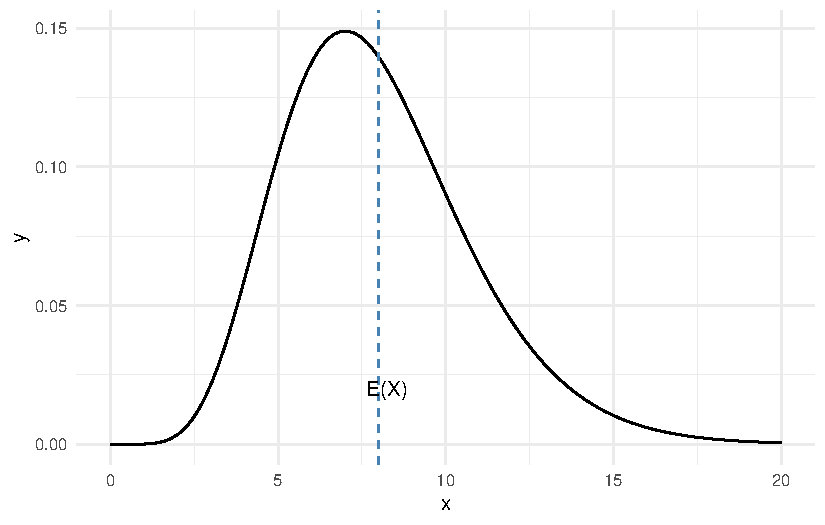
\includegraphics[keepaspectratio]{lecture6_files/figure-pdf/gamma-fig-1.pdf}}

}

\caption{Density of a Gamma(8,1) distribution with mean indicated.}

\end{figure}%

\subsection{}\label{section}

\begin{verbatim}
Coordinate system already present.
i Adding new coordinate system, which will replace the
  existing one.
\end{verbatim}

\begin{figure}[H]

{\centering \pandocbounded{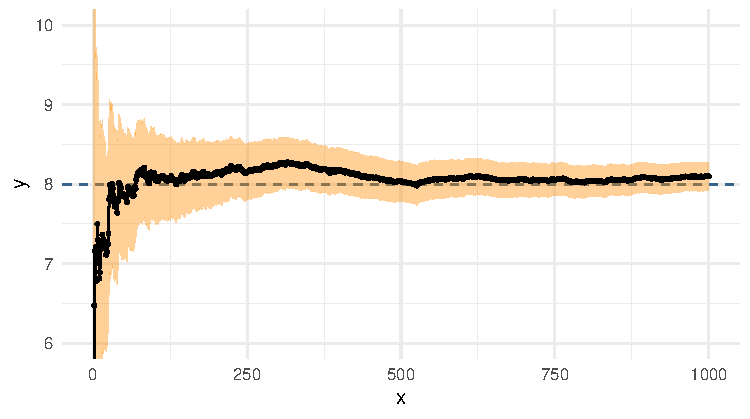
\includegraphics[keepaspectratio]{lecture6_files/figure-pdf/gamma-fig1-1.pdf}}

}

\caption{Convergence of the Monte Carlo estimate of the mean of a
Gamma(8,1) distribution.}

\end{figure}%

\subsection{Choosing the Sample Size}\label{choosing-the-sample-size}

Monte Carlo standard errors decrease as \(1 / \sqrt{N}\): halving the
error requires four times as many samples.

\medskip\pause

Use a pilot run to estimate the variance and plan a \alert{fresh run}
with a fixed sample size: \[
  N
  \approx \left( \frac{1.96\,\hat{\sigma}_{\mathrm{pilot}}}{\varepsilon} \right)^2.
\]

. . .

This targets a 95\% confidence-interval half-width of \(\varepsilon\).

\pdfpcnote{
Round the planned sample size up to an integer. Use independent samples for the
fresh run, fixing its size before generating them. This is approximate
planning: the pilot variance estimate and the normal approximation can be
inaccurate, so the requested precision is not guaranteed. Repeatedly checking
an ordinary confidence interval and stopping when it is narrow does not
guarantee coverage at the resulting data-dependent stopping time.
}

\subsection{Importance Sampling}\label{importance-sampling-1}

When we are only interested in Monte Carlo integration, we do not need
to sample from the target distribution.

. . .

\subsubsection{Basic Idea}\label{basic-idea}

Some regions of the target distribution are often more important than
others.

\medskip\pause

So let's \alert{oversample} these regions, but correct for this by
\alert{weighting} the samples.

\medskip\pause

We want to find \(\mu = \operatorname{E}h(X)\). Observe that \[
  \mu = \int h(x) f(x) \ \mathrm{d}x
      = \int h(x) \frac{f(x)}{g(x)} g(x) \ \mathrm{d}x
      = \int h(x) w^*(x) g(x) \ \mathrm{d}x
\] whenever \(g\) is a density satisfying \[
  g(x) = 0 \Rightarrow f(x) = 0.
\]

\subsection{Weights}\label{weights}

With \(X_1, \ldots, X_N\) i.i.d. with density \(g\), define the
\emph{weights} \[
  w^*(X_i) = \frac{f(X_i)}{g(X_i)}.
\]

. . .

\(g\) is the \emph{importance} density and \(f/g\) is called the
\emph{likelihood ratio}.

. . .

\subsubsection{Estimator}\label{estimator}

\[
  \hat{\mu}_{\mathrm{IS}}^* := \frac{1}{N} \sum_{i=1}^N h(X_i)w^*(X_i).
\]

It has mean \(\mu\).

\subsection{}\label{section-1}

\begin{figure}[H]

{\centering \pandocbounded{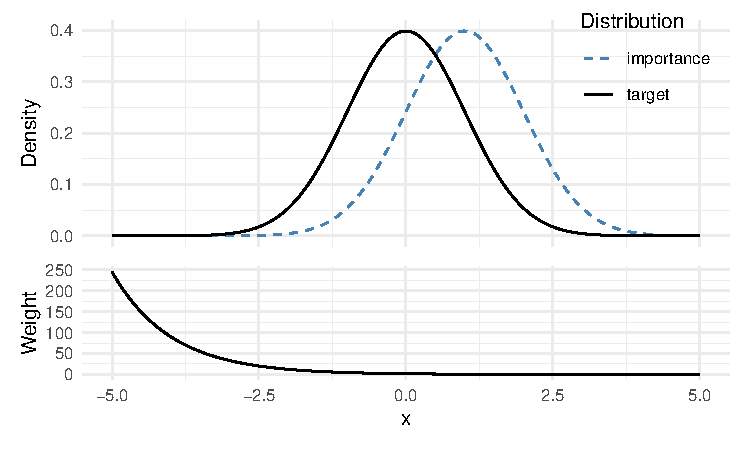
\includegraphics[keepaspectratio]{lecture6_files/figure-pdf/importance-sampling-plot-1.pdf}}

}

\caption{Target and importance densities with corresponding importance
weights.}

\end{figure}%

\subsection{Gamma Importance Sampling}\label{gamma-importance-sampling}

Use \(X = 10 + 3T\), where \(T \sim t_3\). This proposal has heavier
tails than the Gamma target.

\begin{Shaded}
\begin{Highlighting}[]
\NormalTok{B }\OtherTok{\textless{}{-}} \DecValTok{1000}
\NormalTok{t }\OtherTok{\textless{}{-}} \FunctionTok{rt}\NormalTok{(B, }\AttributeTok{df =} \DecValTok{3}\NormalTok{)}
\NormalTok{x }\OtherTok{\textless{}{-}} \DecValTok{10} \SpecialCharTok{+} \DecValTok{3} \SpecialCharTok{*}\NormalTok{ t}
\NormalTok{g\_x }\OtherTok{\textless{}{-}} \FunctionTok{dt}\NormalTok{(t, }\AttributeTok{df =} \DecValTok{3}\NormalTok{) }\SpecialCharTok{/} \DecValTok{3}
\NormalTok{w\_star }\OtherTok{\textless{}{-}} \FunctionTok{dgamma}\NormalTok{(x, }\DecValTok{8}\NormalTok{) }\SpecialCharTok{/}\NormalTok{ g\_x}
\NormalTok{cum\_mean }\OtherTok{\textless{}{-}} \FunctionTok{cumsum}\NormalTok{(x }\SpecialCharTok{*}\NormalTok{ w\_star)}
\NormalTok{mu\_hat\_IS }\OtherTok{\textless{}{-}}\NormalTok{ cum\_mean }\SpecialCharTok{/}\NormalTok{ (}\DecValTok{1}\SpecialCharTok{:}\NormalTok{B)}
\NormalTok{mu\_hat\_IS[B]}
\end{Highlighting}
\end{Shaded}

\begin{verbatim}
[1] 7.946
\end{verbatim}

Close to the theoretical value (8).

. . .

\pandocbounded{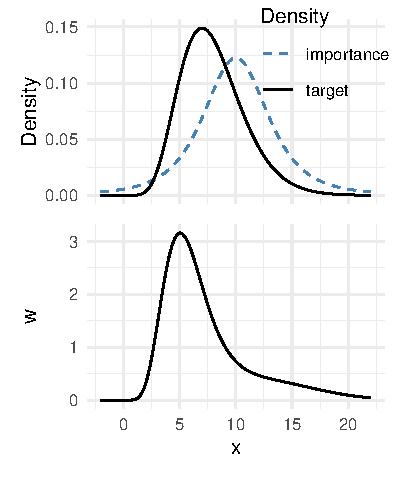
\includegraphics[keepaspectratio]{lecture6_files/figure-pdf/gammasim-fig-1.pdf}}

\subsection{}\label{section-2}

\begin{figure}[H]

{\centering \pandocbounded{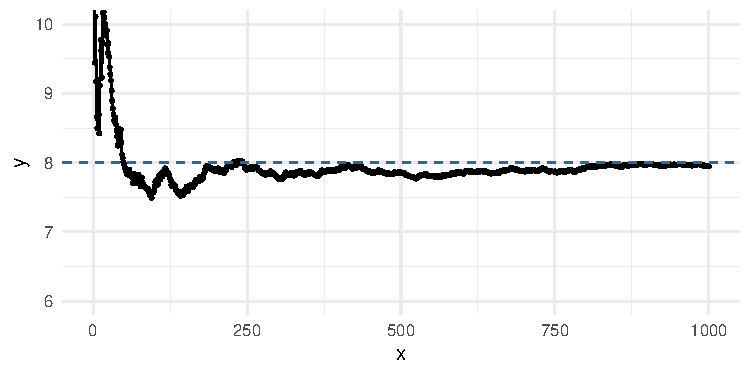
\includegraphics[keepaspectratio]{lecture6_files/figure-pdf/gamma-IS-fig1-1.pdf}}

}

\caption{Convergence of the importance sampling estimate of the mean of
a Gamma(8,1) distribution using a Student-t proposal with 3 degrees of
freedom, location 10, and scale 3.}

\end{figure}%

\subsection{Importance Sampling
Variance}\label{importance-sampling-variance}

Again by the LLN, assuming \(\operatorname{E}_f|h(X)| < \infty\), \[
  \hat{\mu}_{\mathrm{IS}}^* \rightarrow \operatorname{E}h(X_1) w^*(X_1)
                            = \mu \quad \text{as } N \to \infty.\pause
\] If \(\sigma^{*2}_{\mathrm{IS}} < \infty\), the CLT gives \[
  \hat{\mu}_{\mathrm{IS}}^* \overset{\mathrm{approx}}
  \sim \mathcal{N}(\mu, \sigma^{*2}_{\mathrm{IS}} / N)
\] where \[
  \sigma^{*2}_{\mathrm{IS}} = \V \big( h(X_1)w^*(X_1)\big)
                            = \int (h(x) w^*(x) - \mu)^2 g(x) \ \mathrm{d}x.
\]

\subsection{Importance Sampling
Variance}\label{importance-sampling-variance-1}

The IS variance can be estimated analogously to the MC variance, \[
  \hat{\sigma}^{*2}_{\mathrm{IS}}
  = \frac{1}{N - 1} \sum_{i=1}^N (h(X_i)w^*(X_i) - \hat{\mu}_{\mathrm{IS}}^*)^2.
\]

. . .

An approximate 95\% confidence interval is \[
  \hat{\mu}^*_{\mathrm{IS}}
  \pm 1.96 \frac{\hat{\sigma}^*_{\mathrm{IS}}}{\sqrt{N}}.
\]

\medskip\pause

We may have \(\sigma^{*2}_{\mathrm{IS}} > \sigma^2_{\mathrm{MC}}\) or
\(\sigma^{*2}_{\mathrm{IS}} < \sigma^2_{\mathrm{MC}}\) depending on
\(h\) and \(g\).

. . .

\subsubsection{Goal}\label{goal}

Choose \(g\) so that \(|h(x)| w^*(x)\) becomes as constant as possible.

\subsection{Gamma Importance
Sampling}\label{gamma-importance-sampling-1}

\begin{Shaded}
\begin{Highlighting}[]
\NormalTok{sigma\_hat\_IS }\OtherTok{\textless{}{-}} \FunctionTok{sd}\NormalTok{(x }\SpecialCharTok{*}\NormalTok{ w\_star)}
\NormalTok{sigma\_hat\_IS}
\end{Highlighting}
\end{Shaded}

\begin{verbatim}
[1] 4.216
\end{verbatim}

. . .

\begin{figure}[H]

{\centering \pandocbounded{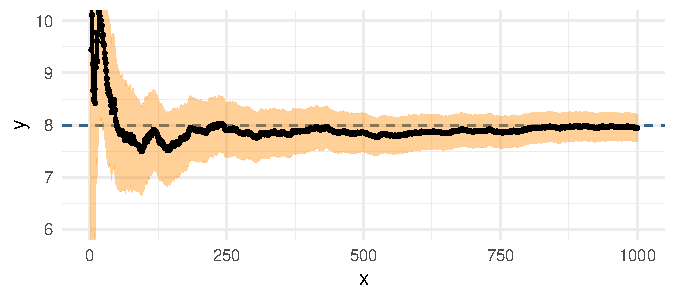
\includegraphics[keepaspectratio]{lecture6_files/figure-pdf/gamma-IS-fig2-1.pdf}}

}

\caption{Gamma mean estimate with approximate pointwise 95\% intervals.}

\end{figure}%

\subsection{Accounting for the
Integrand}\label{accounting-for-the-integrand}

Suppose we want to estimate \[
  \operatorname{E}(X^4) = \int x^4 f(x) \ \mathrm{d}x = 3
\] where \(f(x)\) is the standard normal density.

\medskip\pause

Direct Monte Carlo samples from \(f\), placing most draws near zero.

\medskip\pause

The \alert{integrand} \(x^4f(x)\) peaks at \(x = \pm2\) and decays to
zero in the far tails. We want more draws around those peaks.

\medskip\pause

Try a wider Gaussian: \(g = \mathcal{N}(0,4)\), with standard deviation
\(2\). This puts more mass near \(\pm2\) and reduces the variance of
\(X^4f(X)/g(X)\).

\pdfpcnote{
The proposal should account for the shape of the integrand. Nonlinearity alone
does not tell us which proposal to choose. Differentiating x^4 f(x) gives
x^3 (4 - x^2) f(x), so the two maxima are at -2 and 2. The wider Gaussian is a
simple approximation to this shape; it is not the optimal proposal. The next
two slides illustrate the improvement and give the ideal density.
}

\subsection{}\label{section-3}

\begin{figure}[H]

{\centering \pandocbounded{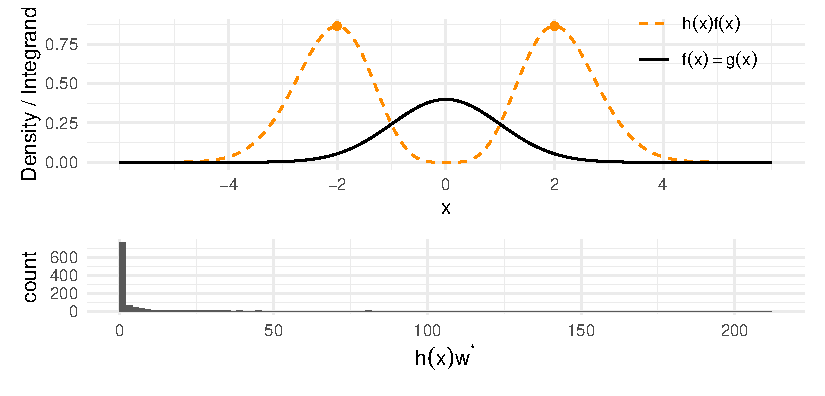
\includegraphics[keepaspectratio]{lecture6_files/figure-pdf/is-normal-plot-1.pdf}}

}

\caption{Direct MC: \(g = f = \mathcal{N}(0,1)\).}

\end{figure}%

\begin{figure}[H]

{\centering \pandocbounded{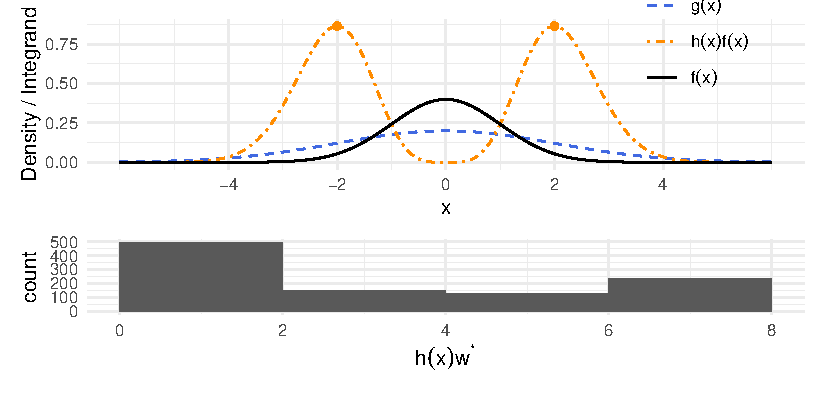
\includegraphics[keepaspectratio]{lecture6_files/figure-pdf/is-wide-normal-plot-1.pdf}}

}

\caption{Importance sampling: \(g = \mathcal{N}(0,4)\).}

\end{figure}%

. . .

For the same \(N\), the estimator variances are \[
  \V(\hat\mu_{\mathrm{MC}}) = \frac{96}{N},
  \qquad
  \V(\hat\mu_{\mathrm{IS}}^*) \approx \frac{7.93}{N}.
\]

\pdfpcnote{
Each histogram shows 1000 weighted contributions, with bin width 2. The
horizontal scales differ. Direct MC contributions are X^4, while the wider
Gaussian gives 2 X^4 exp(-3 X^2 / 8), which is bounded above by about 7.70.
The variances shown are theoretical, not estimates from these histograms:
Var under f of X^4 is E under f of X^8 minus 9 = 105 - 9 = 96.
For g = N(0,4), the second moment is
210 / (7/4)^{9/2}, giving variance approximately 7.925756.
The wider Gaussian reduces variance by a factor of about 12.
}

\subsection{The Ideal Importance
Density}\label{the-ideal-importance-density}

For \(0 < \operatorname{E}_f|h(X)| < \infty\), the variance-minimizing
density for ordinary IS is \[
  g_{\mathrm{opt}}(x) = \frac{|h(x)|f(x)}{\int |h(u)|f(u)\,\mathrm{d}u}.
\]

. . .

If \(h \geq 0\), then \(g_{\mathrm{opt}} = hf / \mu\). Every draw gives
\[
  \frac{h(X)f(X)}{g_{\mathrm{opt}}(X)} = \mu, \qquad X \sim g_{\mathrm{opt}},
\] so the estimator has \alert{zero variance}.

\medskip\pause

But evaluating these weights requires the normalizing constant \(\mu\),
the integral we want. Use the shape of \(|h|f\) to guide a practical
proposal.

\pdfpcnote{
Ordinary IS only requires proposal support wherever the integrand is nonzero.
For sign-changing h, the optimal proposal still minimizes variance, but the
weighted contributions generally have different signs and the variance is not
zero. This result is for ordinary IS, not self-normalized IS.
}

\subsection{Normalized Weights}\label{normalized-weights}

If \(f = c^{-1} q\) with \(c\) unknown\footnote{For instance common in
  Bayesian statistics.} then \[
  c = \int q(x) \ \mathrm{d}x = \int \frac{q(x)}{g(x)} g(x) \ \mathrm{d}x.
\]

. . .

And \[
  \mu
  = \frac{\int h(x) w^*(x) g(x) \ \mathrm{d}x}{\int w^*(x) g(x) \ \mathrm{d}x},
\] where \[
  w^*(x) = \frac{q(x)}{g(x)}.
\]

\pdfpcnote{
Note that g is still the normalized density.
}

\subsection{IS with Normalized
Weights}\label{is-with-normalized-weights}

An importance sampling estimate of \(\mu\) is thus \[
  \hat{\mu}_{\mathrm{IS}}
  = \frac{\sum_{i=1}^N h(X_i) w^*(X_i)}{\sum_{i=1}^N w^*(X_i)} \pause
  = \sum_{i=1}^N h(X_i) w(X_i),
\] where \(w^*(X_i) = q(X_i) / g(X_i)\) and \[
  w(X_i) = \frac{w^*(X_i)}{\sum_{i=1}^N w^*(X_i)}
\] are the \emph{normalized weights}.

\medskip\pause

This works regardless of the normalizing constant \(c\), and also if an
unnormalized proposal density is used in the weights.

\medskip\pause

The estimator is generally biased for finite \(N\), but is consistent
under the support and integrability assumptions.

\subsection{Gamma Sampling with Normalized
Weights}\label{gamma-sampling-with-normalized-weights}

Ignore the normalizing constants of the Gamma target and proposal
\(10 + 3T\), \(T \sim t_3\). Set \(w^*(x) = 0\) for \(x \leq 0\), and
otherwise use \[
  w^*(x) = x^7 e^{-x} \left( 1 + \frac{(x - 10)^2}{27} \right)^2.
\]

. . .

\begin{Shaded}
\begin{Highlighting}[]
\NormalTok{B }\OtherTok{\textless{}{-}} \DecValTok{1000}
\NormalTok{x }\OtherTok{\textless{}{-}} \DecValTok{10} \SpecialCharTok{+} \DecValTok{3} \SpecialCharTok{*} \FunctionTok{rt}\NormalTok{(B, }\AttributeTok{df =} \DecValTok{3}\NormalTok{)}
\NormalTok{w\_star }\OtherTok{\textless{}{-}} \FunctionTok{numeric}\NormalTok{(B)}
\NormalTok{x\_pos }\OtherTok{\textless{}{-}}\NormalTok{ x[x }\SpecialCharTok{\textgreater{}} \DecValTok{0}\NormalTok{]}
\NormalTok{w\_star[x }\SpecialCharTok{\textgreater{}} \DecValTok{0}\NormalTok{] }\OtherTok{\textless{}{-}} \FunctionTok{exp}\NormalTok{(}
  \DecValTok{2} \SpecialCharTok{*} \FunctionTok{log1p}\NormalTok{((x\_pos }\SpecialCharTok{{-}} \DecValTok{10}\NormalTok{)}\SpecialCharTok{\^{}}\DecValTok{2} \SpecialCharTok{/} \DecValTok{27}\NormalTok{) }\SpecialCharTok{{-}}\NormalTok{ x\_pos }\SpecialCharTok{+} \DecValTok{7} \SpecialCharTok{*} \FunctionTok{log}\NormalTok{(x\_pos)}
\NormalTok{)}

\NormalTok{mu\_hat\_IS }\OtherTok{\textless{}{-}} \FunctionTok{cumsum}\NormalTok{(x }\SpecialCharTok{*}\NormalTok{ w\_star) }\SpecialCharTok{/} \FunctionTok{cumsum}\NormalTok{(w\_star)}
\NormalTok{mu\_hat\_IS[B] }\CommentTok{\# Theoretical value 8}
\end{Highlighting}
\end{Shaded}

\begin{verbatim}
[1] 8.124
\end{verbatim}

\subsection{}\label{section-4}

\begin{figure}[H]

{\centering \pandocbounded{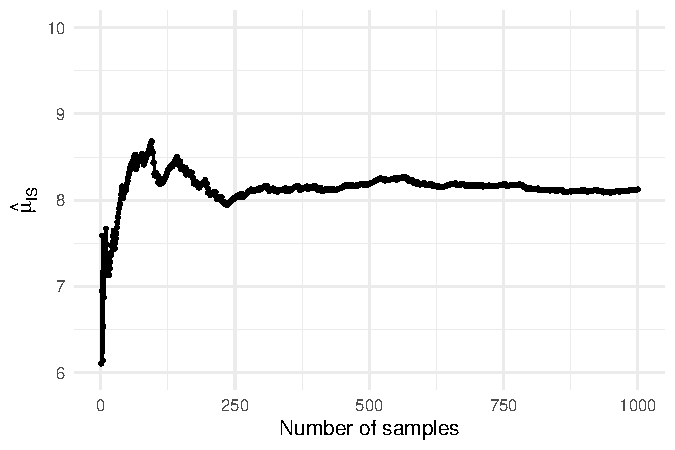
\includegraphics[keepaspectratio]{lecture6_files/figure-pdf/gamma-ISw-fig1-1.pdf}}

}

\caption{Convergence of the importance sampling estimate of the mean of
a Gamma(8,1) distribution using normalized weights.}

\end{figure}%

\subsection{Variance for IS with Normalized
Weights}\label{variance-for-is-with-normalized-weights}

Let \(w_i = w(X_i)\) be the normalized weights. If \(w^*(X)\) and
\(h(X)w^*(X)\) have finite variances, the \(\Delta\)-method gives the
standard error estimate \[
  \widehat{\mathrm{se}}(\hat{\mu}_{\mathrm{IS}})
  = \sqrt{\frac{N}{N - 1} \sum_{i=1}^N w_i^2 \big(h(X_i) - \hat{\mu}_{\mathrm{IS}}\big)^2}.
\]

This accounts for uncertainty in both the weighted sum and the sum of
weights.

\medskip\pause

An approximate 95\% confidence interval is \[
  \hat{\mu}_{\mathrm{IS}}
  \pm 1.96\,\widehat{\mathrm{se}}(\hat{\mu}_{\mathrm{IS}}).
\]

\medskip\pause

Normalizing constants cancel.

\pdfpcnote{
The factor N/(N-1) matches the sample-variance convention used earlier.
Equivalently, compute the sample standard deviation of
w-star times (h minus mu-hat), divide by the mean unnormalized weight,
and then divide by the square root of N.
}

\subsection{Gamma Normalized Weights: Standard
Error}\label{gamma-normalized-weights-standard-error}

\begin{Shaded}
\begin{Highlighting}[]
\NormalTok{w }\OtherTok{\textless{}{-}}\NormalTok{ w\_star }\SpecialCharTok{/} \FunctionTok{sum}\NormalTok{(w\_star)}
\NormalTok{weighted\_residuals }\OtherTok{\textless{}{-}}\NormalTok{ w }\SpecialCharTok{*}\NormalTok{ (x }\SpecialCharTok{{-}}\NormalTok{ mu\_hat\_IS[B])}
\NormalTok{se\_hat\_IS }\OtherTok{\textless{}{-}} \FunctionTok{sqrt}\NormalTok{(B }\SpecialCharTok{/}\NormalTok{ (B }\SpecialCharTok{{-}} \DecValTok{1}\NormalTok{) }\SpecialCharTok{*} \FunctionTok{sum}\NormalTok{(weighted\_residuals}\SpecialCharTok{\^{}}\DecValTok{2}\NormalTok{))}
\NormalTok{se\_hat\_IS}
\end{Highlighting}
\end{Shaded}

\begin{verbatim}
[1] 0.1025
\end{verbatim}

. . .

\begin{figure}[H]

{\centering \pandocbounded{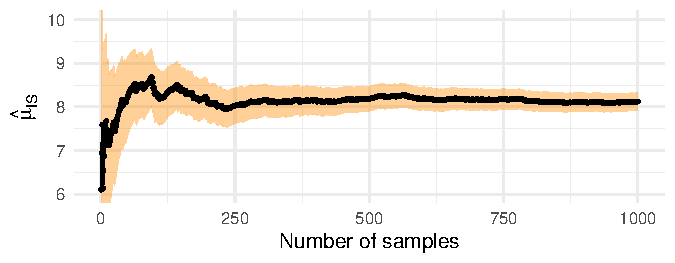
\includegraphics[keepaspectratio]{lecture6_files/figure-pdf/gamma-ISw-fig2-1.pdf}}

}

\caption{Gamma mean estimate with approximate pointwise 95\% intervals.}

\end{figure}%

\subsection{When to Use Importance
Sampling?}\label{when-to-use-importance-sampling}

\subsubsection{Rare Events}\label{rare-events}

Estimating probabilities or expectations involving rare events.

. . .

\subsubsection{High-Variance Monte
Carlo}\label{high-variance-monte-carlo}

Importance sampling can reduce variance by focusing samples where the
integrand is large.

. . .

\subsubsection{Difficult-to-Sample
Targets}\label{difficult-to-sample-targets}

When direct sampling from the target distribution is hard, but sampling
from a related importance distribution is easy.

\subsection{Poor Importance
Distribution}\label{poor-importance-distribution}

If the importance distribution assigns little mass to important regions,
weighted contributions can be highly variable and estimates unreliable.

\medskip\pause

\subsubsection{Remedies}\label{remedies}

More samples may help with poor overlap. They cannot repair missing
support: if \(g = 0\) where \(hf \neq 0\), ordinary IS misses part of
the integral.

\medskip\pause

Redesign the importance density to cover the required support and put
more mass where the integrand is large. Self-normalized IS must cover
the target support, including where \(h = 0\).

\subsection{Diagnostics for Importance
Sampling}\label{diagnostics-for-importance-sampling}

\subsubsection{Weight Distribution}\label{weight-distribution}

Plot the weights and weighted integrand values to identify extreme
contributions.

. . .

\subsubsection{Effective Sample Size
(ESS)}\label{effective-sample-size-ess}

ESS summarizes weight concentration. A high ESS cannot rule out missed
regions.

. . .

\subsubsection{Coefficient of Variation
(CV)}\label{coefficient-of-variation-cv}

CV quantifies the relative variability of the weights.

. . .

\subsubsection{Comparison with Standard Monte
Carlo}\label{comparison-with-standard-monte-carlo}

Comparing with standard Monte Carlo shows whether importance sampling
actually improves efficiency.

\subsection{Weight Degeneracies}\label{weight-degeneracies}

Suppose that \[
  X \sim \mathcal{N}(0, I_{2})
\] and that we want to estimate \(\operatorname{E}(h(X))\) where
\(h(X)\) is large near the origin.

\medskip\pause

If we use an importance density \(g(x)\) from \[
  \mathcal{N}(\mu, I_{2})
\] with large \(\|\mu\|\), most samples are far from the origin, so
\(h(X)\) is nearly zero and weights are highly variable.

\begin{verbatim}
Warning: package 'mvtnorm' was built under R version 4.6.1
\end{verbatim}

\begin{figure}[H]

{\centering \pandocbounded{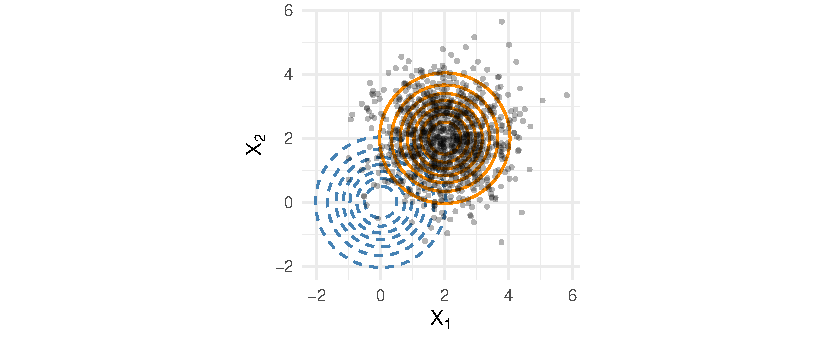
\includegraphics[keepaspectratio]{lecture6_files/figure-pdf/poor-importance-demo-1.pdf}}

}

\caption{Target (blue) and importance (orange) densities with samples
from the importance distribution.}

\end{figure}%

\subsection{}\label{section-5}

\begin{verbatim}
`stat_bin()` using `bins = 30`. Pick better value
`binwidth`.
\end{verbatim}

\begin{figure}[H]

{\centering \pandocbounded{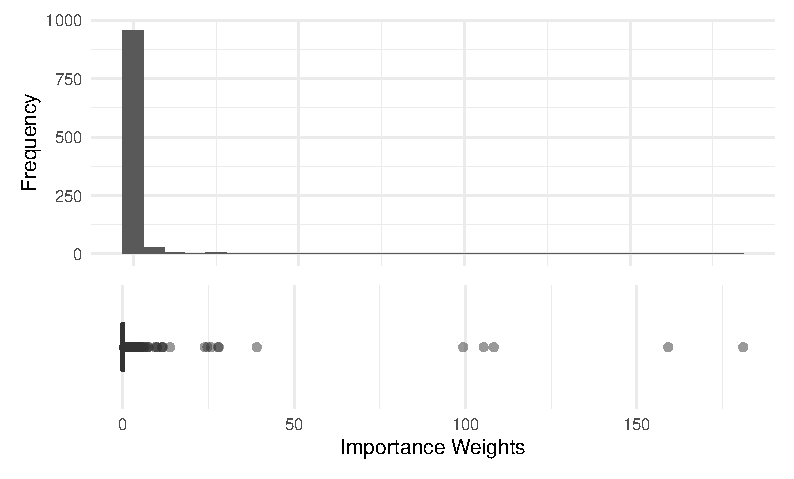
\includegraphics[keepaspectratio]{lecture6_files/figure-pdf/weight-degeneracy-plot-1.pdf}}

}

\caption{Histogram and boxplot of importance weights, showing weight
degeneracy.}

\end{figure}%

\pdfpcnote{
This indicates weight degeneracy and poor sampling efficiency.
}

\subsection{Effective Sample Size
(ESS)}\label{effective-sample-size-ess-1}

The weight-based effective sample size (ESS) summarizes how evenly the
total weight is distributed across samples: \[
  \mathrm{ESS}
  = \frac{1}{\sum_{i=1}^N w_i^2}
  = \frac{\left( \sum_{i=1}^N w^*_i \right)^2}{\sum_{i=1}^N ({w^*_i})^2}
\] where \(w_i\) are the \alert{normalized} importance weights.

\medskip\pause

If all weights are equal, \(\mathrm{ESS} = N\). If one weight dominates,
\(\mathrm{ESS} \approx 1\), which warns of possible instability.

. . .

\subsubsection{Bivariate Normal Example}\label{bivariate-normal-example}

For the bivariate example, with get an ESS of about 14 out of
\(N = 1000\) samples.

\subsection{Coefficient of Variation
(CV)}\label{coefficient-of-variation-cv-1}

The coefficient of variation (CV) of the weights measures their relative
variability.

\medskip\pause

It is defined as \[
  \mathrm{CV}
  = \frac{\sqrt{\frac{1}{N} \sum_{i=1}^N (w_i - \bar{w})^2}}{\bar{w}}
\] where \(\bar{w} = \frac{1}{N} \sum_{i=1}^N w_i\) is the mean weight.

. . .

\subsubsection{Interpretation}\label{interpretation}

A high CV indicates uneven weights, which can make estimates unstable.

\medskip\pause

CV near 0 means nearly uniform weights. Even CV below 1
(\(\mathrm{ESS} > N/2\)) does not guarantee accuracy: the integrand
matters, and samples can miss important regions.

. . .

\subsubsection{Connection to ESS}\label{connection-to-ess}

There is a direct relationship between ESS and CV: \[
  \mathrm{ESS} = \frac{N}{1 + \mathrm{CV}^2}.
\]

\subsection{Choosing the Importance
Distribution}\label{choosing-the-importance-distribution}

We want low-variance estimates of \[
  I = \int h(x) f(x) \ \mathrm{d}x
\]

. . .

The importance distribution determines the weights \[
  w^*(x) = \frac{f(x)}{g(x)}
\] but ordinary IS variance depends on \(h(X)w^*(X)\), not just the
weights. For self-normalized IS, the asymptotic variance depends on
\((h(X) - \mu)w^*(X)\).

\subsection{Principles for Choosing the Importance
Distribution}\label{principles-for-choosing-the-importance-distribution}

\subsubsection{Cover the Support}\label{cover-the-support}

Require \(g(x) > 0\) wherever \(|h(x)|f(x) > 0\) for ordinary IS, and
wherever \(f(x) > 0\) for self-normalized IS, up to sets of measure
zero.

. . .

\subsubsection{Match the Bulk}\label{match-the-bulk}

For ordinary IS, put more mass where \(|h(x)|f(x)\) is large. For
self-normalized IS, the corresponding quantity is \(|h(x) - \mu|f(x)\).

. . .

\subsubsection{Give it Heavy-Enough
Tails}\label{give-it-heavy-enough-tails}

Use tails heavy enough that the weighted contributions have finite
variance. Heavier tails than the target are often a useful safeguard.

\subsection{Common Strategies}\label{common-strategies}

\subsubsection{Exponential Tilting}\label{exponential-tilting}

Multiply the target density by an exponential factor to favor a
rare-event region.

. . .

\subsubsection{Laplace Approximation}\label{laplace-approximation}

Use a Gaussian approximation centered at the mode of the target
distribution.

. . .

\subsubsection{Adaptive Importance
Sampling}\label{adaptive-importance-sampling}

Iteratively refine the importance distribution based on pilot runs.

. . .

\subsubsection{Mixture and Defensive
Proposals}\label{mixture-and-defensive-proposals}

Combine components to capture multiple modes. A defensive component
covers the support and controls the tails of the weighted contributions.

\subsection{A Rare Event: No Hits}\label{a-rare-event-no-hits}

For \(Z \sim \mathcal{N}(0,1)\), estimate \[
  p = P(Z > 4) \approx 3.17 \times 10^{-5}.
\]

\begin{Shaded}
\begin{Highlighting}[]
\NormalTok{n\_rare }\OtherTok{\textless{}{-}} \DecValTok{10000}
\NormalTok{rare\_hits }\OtherTok{\textless{}{-}} \FunctionTok{rnorm}\NormalTok{(n\_rare) }\SpecialCharTok{\textgreater{}} \DecValTok{4}
\FunctionTok{mean}\NormalTok{(rare\_hits)}
\end{Highlighting}
\end{Shaded}

\begin{verbatim}
[1] 0
\end{verbatim}

. . .

This is typical: with \(N = 10{,}000\), \[
  P(\text{no exceedances}) = (1 - p)^N \approx 0.729.
\]

The empirical standard error is also zero. We have missed the event, not
established that its probability is zero.

\subsection{A Rare Event: Exponential
Tilting}\label{a-rare-event-exponential-tilting}

For the standard normal density \(f = \phi\), an
\alert{exponential tilt} shifts the mean: \[
  g_\theta(x) = e^{\theta x-\theta^2 / 2} f(x) = \phi(x - \theta).
\]

Choose \(\theta = 4\): \(X_i \sim \mathcal{N}(4,1)\) and
\(w^*(x) = f(x) / g_4(x) = e^{8-4x}\).

\begin{figure}[H]

{\centering \pandocbounded{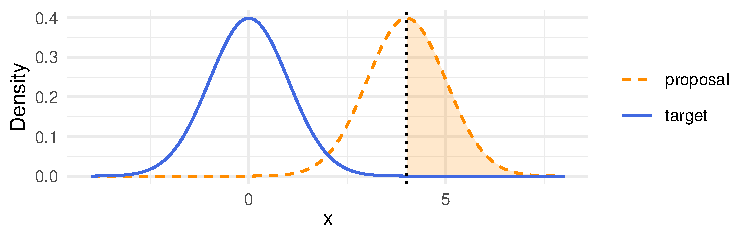
\includegraphics[keepaspectratio]{lecture6_files/figure-pdf/rare-event-proposal-1.pdf}}

}

\caption{Target and proposal densities for the rare-event example.}

\end{figure}%

. . .

\[
  \hat{p}_{\mathrm{IS}}
  = \frac{1}{N} \sum_{i=1}^N \mathbf{1}\{X_i > 4\}\,e^{8-4X_i}.
\]

\pdfpcnote{
Exponential tilting multiplies the density by exp(theta times x) and divides
by the moment-generating function. For a standard normal, this normalizing
constant is exp(theta squared divided by 2). Completing the square gives a
normal distribution with mean theta and variance 1. At theta = 4, half the
proposal draws exceed 4. Shifting a general density need not be an exponential
tilt.

The ideal proposal is the standard normal conditional on exceeding 4. Its
normalizing constant is p. The shifted normal is a simple approximation that
makes exceedances common and has an evaluable, normalized density.
}

\subsection{A Rare Event: Repeated
Runs}\label{a-rare-event-repeated-runs}

500 independent runs per method, with \(N = 10{,}000\) draws per run.

\begin{figure}[H]

{\centering \pandocbounded{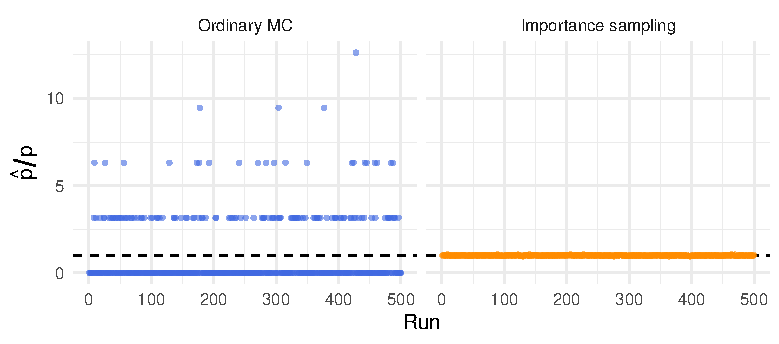
\includegraphics[keepaspectratio]{lecture6_files/figure-pdf/rare-event-comparison-1.pdf}}

}

\caption{Estimates of the rare-event probability \(p\) from 500
independent runs of ordinary Monte Carlo and importance sampling.}

\end{figure}%

The dashed line is the truth. MC returned zero in 73.2\% of runs.

\medskip\pause

IS had about 91 times smaller empirical standard deviation at the same
sample size.

\subsection{Laplace Approximation}\label{laplace-approximation-1}

\subsubsection{Basic Idea}\label{basic-idea-1}

Take a Gaussian approximation of the target density at its mode \(x^*\)
as the importance distribution.

. . .

\subsubsection{Motivation}\label{motivation}

The connection comes from the second-order Taylor expansion of
\(\log f(x)\) at an interior mode \(x^*\), \[
  \log f(x) \approx \log f(x^*) - \frac{1}{2}(x - x^*)^T \Lambda (x - x^*)
\] where \(\Lambda\) is the Hessian of \(-\log f(x)\) at \(x^*\),
assumed positive definite.

\medskip\pause

Exponentiating both sides gives: \[
  f(x)
  \approx f(x^*) \exp\left( -\frac{1}{2}(x - x^*)^T \Lambda (x - x^*) \right)
\]

\subsection{Laplace Approximation}\label{laplace-approximation-2}

\subsubsection{Steps}\label{steps}

\begin{enumerate}
\def\labelenumi{\arabic{enumi}.}
\tightlist
\item
  Find the mode \(x^* = \mathop{\mathrm{\arg\,\max}}_x f(x)\).\pause
\item
  Compute the Hessian \(\Lambda\) of \(-\log f(x)\) at \(x^*\).\pause
\item
  If \(\Lambda\) is positive definite, use
  \(\mathcal{N}(x^*, \Lambda^{-1})\) as the importance distribution.
\end{enumerate}

. . .

\subsubsection{When to Use}\label{when-to-use}

Useful for smooth targets with an approximately Gaussian shape near the
mode. Check the tails before using it for importance sampling.

\subsection{Example: Gamma
Distribution}\label{example-gamma-distribution-1}

The density of the \(\mathrm{Gamma}(3,1)\) distribution is \[
  f(x) = \frac{1}{2} x^2 e^{-x}, \quad x > 0.
\]

. . .

The mode is at \(x^* = 2\) and the Hessian of \(-\log f(x)\) at \(x^*\)
is \[
  \Lambda = \frac{\alpha - 1}{(x^*)^2} = \frac 1 2.
\]

\medskip\pause

So the Laplace approximation is \(\mathcal{N}(2, 2)\), with standard
deviation \(\sqrt{2}\).

\begin{figure}[H]

{\centering \pandocbounded{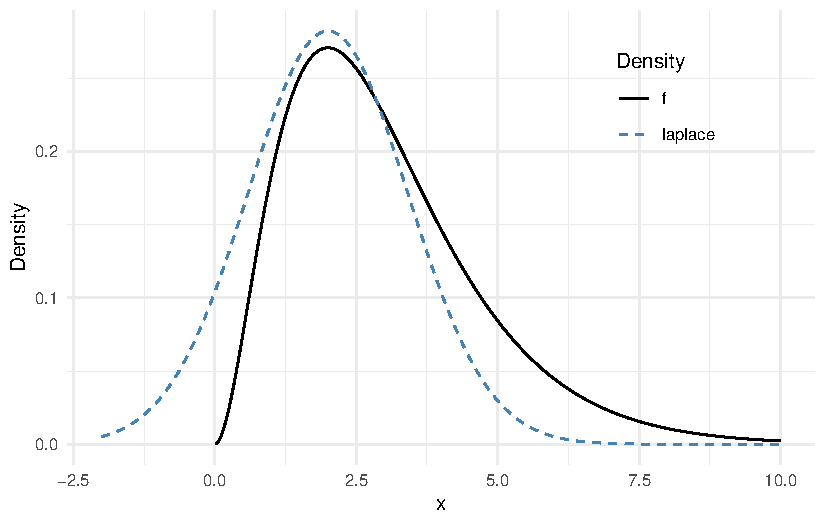
\includegraphics[keepaspectratio]{lecture6_files/figure-pdf/laplace-approx-plot-1.pdf}}

}

\caption{Target (solid black) and Laplace approximation (dashed blue)
densities for a Gamma(3,1) distribution.}

\end{figure}%

\subsection{Adaptive Importance
Sampling}\label{adaptive-importance-sampling-1}

Adaptive importance sampling iteratively refines the importance
distribution based on the samples obtained.

. . .

\subsubsection{Basic Idea}\label{basic-idea-2}

Start with an initial importance distribution and refine it based on
samples and weights.

. . .

\subsubsection{Steps}\label{steps-1}

\begin{enumerate}
\def\labelenumi{\arabic{enumi}.}
\tightlist
\item
  Choose an initial importance distribution \(g_0(x)\) and set
  \(n = 0\).\pause
\item
  Draw samples from the current proposal \(g_n\) and compute
  weights.\pause
\item
  Fit \(g_{n+1}\) using the weighted samples, then increment \(n\).
  \pause
\item
  Repeat steps 2-3 until the proposal stabilizes.
\end{enumerate}

\subsection{Moment-Matching Importance
Sampling}\label{moment-matching-importance-sampling}

One simple adaptive strategy is to use moment-matching to update a
Gaussian importance distribution.

\medskip\pause

At iteration \(n\), draw samples \(x_1, \ldots, x_N \sim g_n(x)\) and
compute weights \[
  w_i^* = \frac{f(x_i)}{g_n(x_i)}.
\]

. . .

Then update the importance distribution parameters as \[
\begin{aligned}
  \mu_{n + 1}      &= \frac{\sum_{i=1}^N w_i^* x_i}{\sum_{i=1}^N w_i^*},\\
  \sigma^2_{n + 1} &= \frac{\sum_{i=1}^N w_i^* (x_i - \mu_{n + 1})^2}{\sum_{i=1}^N w_i^*}.
\end{aligned}
\]

\pdfpcnote{
This can be extended to multivariate targets using weighted covariance.
}

\subsection{}\label{section-6}

\begin{figure}[htpb]
\centering
\multiinclude[<+>][format=pdf,start=1,end=5]{lecture6_files/figure-pdf/adaptive-importance-fig}
\caption{Adaptive importance sampling with a Gaussian proposal.}
\end{figure}

\subsection{Defensive Importance
Sampling}\label{defensive-importance-sampling}

Return to the \(\mathrm{Gamma}(3,1)\) target and estimating
\(\operatorname{E}_f[X] = 3\). The Laplace proposal
\(g_L = \mathcal{N}(2,2)\) has a right tail that is too light: ordinary
IS has \alert{infinite variance}.

\medskip\pause

Add a heavy-tailed component \(g_t\), the density of \(2 + \sqrt{2}T\)
with \(T \sim t_3\): \[
  g_{\mathrm{mix}}(x) = 0.9 g_L(x) + 0.1 g_t(x).
\]

. . .

Since \(g_{\mathrm{mix}} \geq 0.1g_t\), the mixture inherits protection
from the Student-\(t\) tails. For this Gamma mean, it restores
\alert{finite variance}.

\pdfpcnote{
For h(x) = x, the second moment of an ordinary IS contribution is the integral
of x squared times f squared divided by g. For the Gaussian proposal, this
integrand is proportional to x to the sixth power times
exp(x squared divided by 4 minus 3x), whose integral diverges.

The Student-t density decays as x to the minus fourth power, so its second-moment
integrand decays as x to the tenth power times exp(-2x), which is integrable.
Since the mixture is at least 0.1 times the Student-t density, its second moment
is at most ten times the Student-t second moment. This restores finite variance,
although it need not give a smaller variance than direct Monte Carlo.
}

\subsection{}\label{section-7}

\begin{figure}[H]

{\centering \pandocbounded{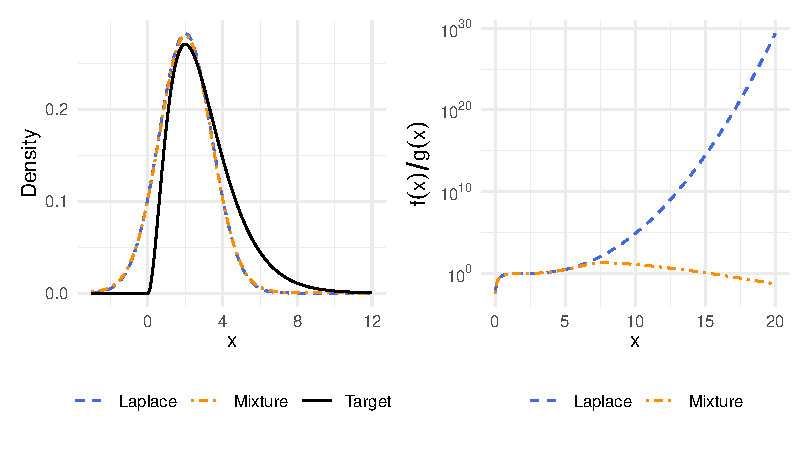
\includegraphics[keepaspectratio]{lecture6_files/figure-pdf/gamma-defensive-fig-1.pdf}}

}

\caption{Gamma(3,1) target and proposals (left); importance weights on a
logarithmic scale (right).}

\end{figure}%

\subsection{Exercise: Von Mises Importance
Sampling}\label{exercise-von-mises-importance-sampling}

\subsubsection{Step 1}\label{step-1}

Estimate the arithmetic mean of the von Mises distribution on
\([-\pi,\pi]\) with \(\mu = 0\) and \(\kappa = 2\). Plot convergence
toward \(\operatorname{E}X = 0\).

\begin{Shaded}
\begin{Highlighting}[]
\NormalTok{dvmises }\OtherTok{\textless{}{-}} \ControlFlowTok{function}\NormalTok{(x, }\AttributeTok{mu =} \DecValTok{0}\NormalTok{, }\AttributeTok{kappa =} \DecValTok{2}\NormalTok{) \{}
  \FunctionTok{ifelse}\NormalTok{(}
    \FunctionTok{abs}\NormalTok{(x) }\SpecialCharTok{\textless{}=}\NormalTok{ pi,}
    \FunctionTok{exp}\NormalTok{(kappa }\SpecialCharTok{*} \FunctionTok{cos}\NormalTok{(x }\SpecialCharTok{{-}}\NormalTok{ mu)) }\SpecialCharTok{/}\NormalTok{ (}\DecValTok{2} \SpecialCharTok{*}\NormalTok{ pi }\SpecialCharTok{*} \FunctionTok{besselI}\NormalTok{(kappa, }\DecValTok{0}\NormalTok{)),}
    \DecValTok{0}
\NormalTok{  )}
\NormalTok{\}}
\end{Highlighting}
\end{Shaded}

. . .

\subsubsection{Step 2}\label{step-2}

Compute the estimate of the mean and its standard error.

. . .

\subsubsection{Step 3}\label{step-3}

Compute the effective sample size and coefficient of variation of the
importance weights. Experiment with different importance densities to
see if you find a better one.

\pdfpcnote{
For nonzero mu, the arithmetic mean on this fixed interval generally differs
from mu, the circular mean direction. Keep mu = 0 for this exercise.
}

\subsection{Solution: Step 1 --- Estimate the
Mean}\label{solution-step-1-estimate-the-mean}

The density is symmetric about zero, so \(x f(x)\) is odd and
\(\operatorname{E}X = \int_{-\pi}^{\pi} x f(x)\,\mathrm{d}x = 0\). Use
the proposal \(g = \mathcal{N}(0,(\pi/2)^2)\) and ordinary IS: \[
  \hat\mu_n = \frac{1}{n}\sum_{i=1}^n X_i w_i^*,
  \qquad w_i^* = \frac{f(X_i)}{g(X_i)}.
\] The target density is normalized, so there is no need to divide by
the sum of weights. Draws outside \([-\pi,\pi]\) receive zero weight and
remain in the sample of size \(n\).

\begin{Shaded}
\begin{Highlighting}[]
\FunctionTok{set.seed}\NormalTok{(}\DecValTok{2026}\NormalTok{)}
\NormalTok{vm\_N }\OtherTok{\textless{}{-}} \DecValTok{10000}
\NormalTok{vm\_x }\OtherTok{\textless{}{-}} \FunctionTok{rnorm}\NormalTok{(vm\_N, }\AttributeTok{sd =}\NormalTok{ pi }\SpecialCharTok{/} \DecValTok{2}\NormalTok{)}
\NormalTok{vm\_weights }\OtherTok{\textless{}{-}} \FunctionTok{dvmises}\NormalTok{(vm\_x) }\SpecialCharTok{/} \FunctionTok{dnorm}\NormalTok{(vm\_x, }\AttributeTok{sd =}\NormalTok{ pi }\SpecialCharTok{/} \DecValTok{2}\NormalTok{)}
\NormalTok{vm\_values }\OtherTok{\textless{}{-}}\NormalTok{ vm\_x }\SpecialCharTok{*}\NormalTok{ vm\_weights}
\NormalTok{vm\_running\_mean }\OtherTok{\textless{}{-}} \FunctionTok{cumsum}\NormalTok{(vm\_values) }\SpecialCharTok{/} \FunctionTok{seq\_len}\NormalTok{(vm\_N)}
\end{Highlighting}
\end{Shaded}

\subsection{Solution: Step 1 ---
Convergence}\label{solution-step-1-convergence}

\begin{figure}[H]

{\centering \pandocbounded{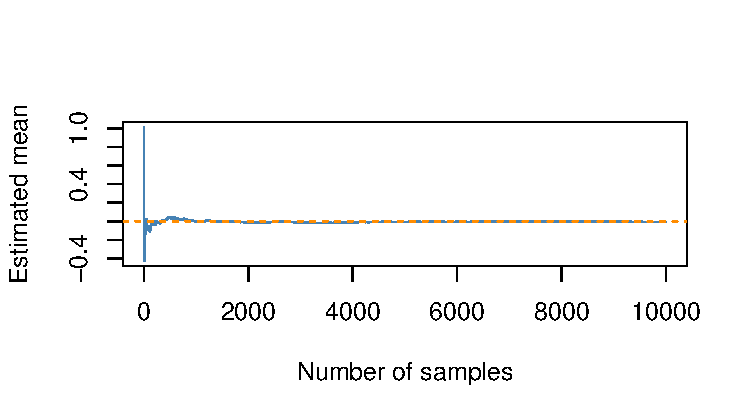
\includegraphics[keepaspectratio]{lecture6_files/figure-pdf/vmises-convergence-1.pdf}}

}

\caption{Running ordinary IS estimate of the von Mises arithmetic mean.}

\end{figure}%

The running estimate approaches zero by the law of large numbers; its
path need not be monotone.

\subsection{Solution: Step 2 --- Standard
Error}\label{solution-step-2-standard-error}

Set \(Y_i = X_i w_i^*\). The estimate is the sample mean of the \(Y_i\),
so \[
  \widehat{\mathrm{se}}(\hat\mu_N)
  = \frac{s_Y}{\sqrt{N}},
  \qquad
  s_Y^2 = \frac{1}{N-1}\sum_{i=1}^N(Y_i-\hat\mu_N)^2.
\] Use the standard deviation of the weighted contributions, not the
sampled \(X_i\) or the weights alone.

\begin{Shaded}
\begin{Highlighting}[]
\NormalTok{vm\_estimate }\OtherTok{\textless{}{-}} \FunctionTok{mean}\NormalTok{(vm\_values)}
\NormalTok{vm\_se }\OtherTok{\textless{}{-}} \FunctionTok{sd}\NormalTok{(vm\_values) }\SpecialCharTok{/} \FunctionTok{sqrt}\NormalTok{(vm\_N)}
\FunctionTok{c}\NormalTok{(}
  \AttributeTok{estimate =}\NormalTok{ vm\_estimate,}
  \AttributeTok{standard\_error =}\NormalTok{ vm\_se,}
  \AttributeTok{lower\_95 =}\NormalTok{ vm\_estimate }\SpecialCharTok{{-}} \FloatTok{1.96} \SpecialCharTok{*}\NormalTok{ vm\_se,}
  \AttributeTok{upper\_95 =}\NormalTok{ vm\_estimate }\SpecialCharTok{+} \FloatTok{1.96} \SpecialCharTok{*}\NormalTok{ vm\_se}
\NormalTok{)}
\end{Highlighting}
\end{Shaded}

\begin{verbatim}
      estimate standard_error       lower_95       upper_95 
     -0.005544       0.007253      -0.019759       0.008672 
\end{verbatim}

\subsection{Solution: Step 3 --- Weight
Diagnostics}\label{solution-step-3-weight-diagnostics}

Using unnormalized weights, calculate \[
  \mathrm{ESS} = \frac{(\sum_i w_i^*)^2}{\sum_i (w_i^*)^2},
  \qquad
  \mathrm{CV} = \frac{\sqrt{N^{-1}\sum_i(w_i^*-\bar w^*)^2}}{\bar w^*}.
\] The CV uses divisor \(N\), as in the lecture; R's \texttt{sd()} uses
\(N-1\).

\begin{Shaded}
\begin{Highlighting}[]
\NormalTok{vm\_diagnostics }\OtherTok{\textless{}{-}} \ControlFlowTok{function}\NormalTok{(x, weights) \{}
\NormalTok{  n }\OtherTok{\textless{}{-}} \FunctionTok{length}\NormalTok{(x)}
  \FunctionTok{data.frame}\NormalTok{(}
    \AttributeTok{estimate =} \FunctionTok{mean}\NormalTok{(x }\SpecialCharTok{*}\NormalTok{ weights),}
    \AttributeTok{SE =} \FunctionTok{sd}\NormalTok{(x }\SpecialCharTok{*}\NormalTok{ weights) }\SpecialCharTok{/} \FunctionTok{sqrt}\NormalTok{(n),}
    \AttributeTok{ESS =} \FunctionTok{sum}\NormalTok{(weights)}\SpecialCharTok{\^{}}\DecValTok{2} \SpecialCharTok{/} \FunctionTok{sum}\NormalTok{(weights}\SpecialCharTok{\^{}}\DecValTok{2}\NormalTok{),}
    \AttributeTok{CV =} \FunctionTok{sqrt}\NormalTok{(}\FunctionTok{mean}\NormalTok{((weights }\SpecialCharTok{{-}} \FunctionTok{mean}\NormalTok{(weights))}\SpecialCharTok{\^{}}\DecValTok{2}\NormalTok{)) }\SpecialCharTok{/} \FunctionTok{mean}\NormalTok{(weights)}
\NormalTok{  )}
\NormalTok{\}}
\NormalTok{vm\_baseline }\OtherTok{\textless{}{-}} \FunctionTok{vm\_diagnostics}\NormalTok{(vm\_x, vm\_weights)}
\NormalTok{vm\_baseline}
\end{Highlighting}
\end{Shaded}

\begin{verbatim}
   estimate       SE  ESS    CV
1 -0.005544 0.007253 6876 0.674
\end{verbatim}

\subsection{Solution: Step 3 --- Compare
Proposals}\label{solution-step-3-compare-proposals}

Try normal proposals with standard deviations \(1\) and \(1.3\), which
concentrate more draws near the target's mode, and
\(\mathrm{Uniform}(-\pi,\pi)\), which covers exactly its support. All
four proposals are positive throughout the target's support.

\begin{Shaded}
\begin{Highlighting}[]
\FunctionTok{set.seed}\NormalTok{(}\DecValTok{2027}\NormalTok{)}
\NormalTok{vm\_x\_normal }\OtherTok{\textless{}{-}} \FunctionTok{rnorm}\NormalTok{(vm\_N, }\AttributeTok{sd =} \DecValTok{1}\NormalTok{)}
\NormalTok{vm\_w\_normal }\OtherTok{\textless{}{-}} \FunctionTok{dvmises}\NormalTok{(vm\_x\_normal) }\SpecialCharTok{/} \FunctionTok{dnorm}\NormalTok{(vm\_x\_normal)}
\NormalTok{vm\_x\_uniform }\OtherTok{\textless{}{-}} \FunctionTok{runif}\NormalTok{(vm\_N, }\SpecialCharTok{{-}}\NormalTok{pi, pi)}
\NormalTok{vm\_w\_uniform }\OtherTok{\textless{}{-}} \FunctionTok{dvmises}\NormalTok{(vm\_x\_uniform) }\SpecialCharTok{/}
  \FunctionTok{dunif}\NormalTok{(vm\_x\_uniform, }\SpecialCharTok{{-}}\NormalTok{pi, pi)}
\NormalTok{vm\_x\_middle }\OtherTok{\textless{}{-}} \FunctionTok{rnorm}\NormalTok{(vm\_N, }\AttributeTok{sd =} \FloatTok{1.3}\NormalTok{)}
\NormalTok{vm\_w\_middle }\OtherTok{\textless{}{-}} \FunctionTok{dvmises}\NormalTok{(vm\_x\_middle) }\SpecialCharTok{/} \FunctionTok{dnorm}\NormalTok{(vm\_x\_middle, }\AttributeTok{sd =} \FloatTok{1.3}\NormalTok{)}

\NormalTok{vm\_comparison }\OtherTok{\textless{}{-}} \FunctionTok{rbind}\NormalTok{(}
\NormalTok{  vm\_baseline,}
  \FunctionTok{vm\_diagnostics}\NormalTok{(vm\_x\_normal, vm\_w\_normal),}
  \FunctionTok{vm\_diagnostics}\NormalTok{(vm\_x\_middle, vm\_w\_middle),}
  \FunctionTok{vm\_diagnostics}\NormalTok{(vm\_x\_uniform, vm\_w\_uniform)}
\NormalTok{)}
\NormalTok{vm\_comparison }\OtherTok{\textless{}{-}} \FunctionTok{data.frame}\NormalTok{(}
  \AttributeTok{proposal =} \FunctionTok{c}\NormalTok{(}
    \StringTok{"Normal, sd = pi/2"}\NormalTok{, }\StringTok{"Normal, sd = 1"}\NormalTok{,}
    \StringTok{"Normal, sd = 1.3"}\NormalTok{, }\StringTok{"Uniform({-}pi, pi)"}
\NormalTok{  ),}
\NormalTok{  vm\_comparison}
\NormalTok{)}
\NormalTok{knitr}\SpecialCharTok{::}\FunctionTok{kable}\NormalTok{(vm\_comparison, }\AttributeTok{digits =} \FunctionTok{c}\NormalTok{(}\DecValTok{0}\NormalTok{, }\DecValTok{5}\NormalTok{, }\DecValTok{5}\NormalTok{, }\DecValTok{0}\NormalTok{, }\DecValTok{3}\NormalTok{), }\AttributeTok{row.names =} \ConstantTok{FALSE}\NormalTok{)}
\end{Highlighting}
\end{Shaded}

{\def\LTcaptype{none} % do not increment counter
\begin{longtable}[]{@{}lrrrr@{}}
\toprule\noalign{}
proposal & estimate & SE & ESS & CV \\
\midrule\noalign{}
\endhead
\bottomrule\noalign{}
\endlastfoot
Normal, sd = pi/2 & -0.00554 & 0.00725 & 6876 & 0.674 \\
Normal, sd = 1 & -0.00261 & 0.00856 & 9372 & 0.259 \\
Normal, sd = 1.3 & -0.00101 & 0.00720 & 7972 & 0.504 \\
Uniform(-pi, pi) & 0.00950 & 0.00802 & 4582 & 1.087 \\
\end{longtable}
}

\subsection{Solution: Step 3 ---
Interpretation}\label{solution-step-3-interpretation}

At the same sample size, the smallest estimated standard error in this
run is obtained with \textbf{Normal, sd = 1.3}. Compare standard errors
to judge precision for this particular mean; proximity of one estimate
to zero can be luck.

Higher ESS and lower CV indicate more even weights, but do not
necessarily give a smaller standard error: that also depends on the
integrand \(h(x)=x\). For ordinary IS the ideal proposal is proportional
to \(|x|f(x)\), rather than just \(f(x)\). Thus concentrating too
tightly around zero can miss useful tail contributions. These
diagnostics are empirical, so repeat the comparison with other seeds or
larger samples before drawing strong conclusions.

\subsection{Summary}\label{summary}

\subsubsection{Monte Carlo Methods}\label{monte-carlo-methods-2}

Estimate integrals and means using random sampling when analytic
solutions are not possible.

. . .

\subsubsection{Importance Sampling}\label{importance-sampling-2}

Focus samples where they matter most, but choose your proposal carefully
to avoid large or variable weights.

. . .

\subsubsection{Diagnostics}\label{diagnostics}

Examine weights, weighted integrand values, and ESS to detect
instability. These checks cannot guarantee accuracy or reveal every
missed region.

. . .

\subsubsection{Picking Importance
Distributions}\label{picking-importance-distributions}

It's hard! But use adaptive and defensive methods to help fix poor
coverage and improve robustness.

\subsection{Next Time}\label{next-time}

\subsubsection{Optimization}\label{optimization}

We introduce optimization methods for minimizing and maximizing
functions.

\medskip\pause

We'll focus on \textbf{convex optimization}, a special class of
optimization problems that are easier to solve and have nice properties.

\lectureappendix

\section{Appendix}\label{appendix}

\subsection{Variance for IS with Normalized
Weights}\label{variance-for-is-with-normalized-weights-1}

Computing the variance of IS with normalized weights is more complicated
because the estimator is a \alert{ratio of random variables}.

\medskip\pause

Write \(c = \operatorname{E}_g[w^*(X)]\). If both \(h(X)w^*(X)\) and
\(w^*(X)\) have finite variances, the multivariate CLT gives \[
  \frac{1}{N} \sum_{i=1}^N \begin{bmatrix} h(X_i) w^*(X_i) \\ w^*(X_i) \end{bmatrix}
  \overset{\mathrm{approx}}{\sim}
  \mathcal{N}\left(
    c \begin{bmatrix} \mu \\ 1\end{bmatrix},
    \frac{1}{N} \begin{bmatrix} \sigma^{2}_{\mathrm{IS}} & \gamma \\ \gamma & \sigma^2_{w^*} \end{bmatrix}
  \right),
\] where \[
\begin{aligned}
  \sigma^2_{\mathrm{IS}} & = \V \big(h(X_1) w^*(X_1)\big) \\
  \gamma & = \mathop{\mathrm{Cov}}(h(X_1) w^*(X_1), w^*(X_1)) \\
  \sigma^2_{w^*} & = \V (w^*(X_1))
\end{aligned}
\]

\subsection{Importance Sampling
Variance}\label{importance-sampling-variance-2}

We can then apply the \(\Delta\)-method with \(t(x, y) = x / y\).

\medskip\pause

Observe that
\(\nabla t(x, y) = \begin{bmatrix} 1 / y \\ -x / y^2 \end{bmatrix}\) ,
whence

\[
  \nabla t(c\mu, c)^T \left(\begin{array}{cc} \sigma^{2}_{\mathrm{IS}} & \gamma \\ \gamma & \sigma^2_{w^*}
  \end{array} \right) \nabla t(c\mu, c) = \frac{\sigma^{2}_{\mathrm{IS}} + \mu^2 \sigma_{w^*}^2 - 2 \mu \gamma}{c^{2}}.
\]

. . .

By the \(\Delta\)-method, \[
  \hat{\mu}_{\mathrm{IS}} \overset{\mathrm{approx}}{\sim} \mathcal{N}\left( \mu, \frac{\sigma^{2}_{\mathrm{IS}} + \mu^2 \sigma_{w^*}^2 - 2 \mu \gamma}{c^2 N} \right).
\]

. . .

Plug in empirical estimates, estimating \(c\) when it is unknown by \[
  \hat{c} = \frac{1}{N} \sum_{i=1}^N w^*(X_i).
\]

If both densities in the weights are unnormalized, \(c\) is the ratio of
their normalizing constants.

\pdfpcnote{
hat(c) is just the MC estimate of c.
}

\subsection{}\label{section-8}

\begin{figure}[H]

{\centering \pandocbounded{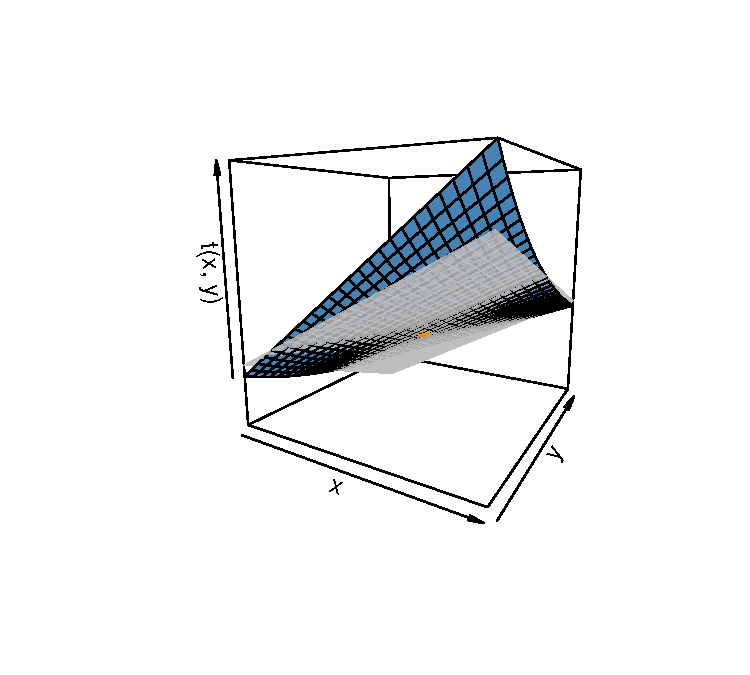
\includegraphics[keepaspectratio]{lecture6_files/figure-pdf/delta-method-plot3D-1.pdf}}

}

\caption{Tangent plane approximation of the function \(t(x,y) = x/y\) at
the point \((2,3)\).}

\end{figure}%




\end{document}
